% 'Notas de aula não oficiais de MS650 e F620' (c) 2012, 2013 by Raniere Silva
% <ra092767@ime.unicamp.br>
%
% 'Notas de aula não oficiais de MS650 e F620' is licensed under a
% Creative Commons Attribution-ShareAlike 3.0 Unported License.
%
% You should have received a copy of the license along with this
% work.  If not, see <http://creativecommons.org/licenses/by-sa/3.0/>.

% Este arquivo inclui o conteúdo de:
%
% * M2S12-9.pdf
% * M2S12-10.pdf
% * M2S12-11.pdf
% * M2S12-12.pdf

\chapter{Transformadas de Fourier}
\subsection{Da série para a Transformada}
Seja a série de Fourier de uma função com período $T = 2L$,
\begin{align*}
    f(x) &= \sum_{n = -\infty}^\infty c_n \exp\left( i n \pi x / L \right), \\
    c_n &= \frac{1}{2L} \int_{-L}^L f(x) \exp\left( -i n \pi x / L \right)
    \id{x}.
\end{align*}
O que desejamos agora é considerar uma função que não seja
necessariamente periódica, ou seja, estender o intervalo para todo o
$\mathbb{R}$ tomando $L \to \infty$. Para isso vamos denotar
\begin{align*}
    K = K(n) &= n \pi / L, \\
    \Delta K &= K(n + 1) - K(n) = \pi / L.
\end{align*}
Então:
\begin{align*}
    f(x) &= \sum_{n = -\infty}^\infty c_n \exp\left( i K(n) x \right) \\
    &= \sum_{n = -\infty}^\infty \left( \frac{c_n L}{\pi} \right) \exp\left(
    i K(n) x \right) \Delta K
\end{align*}
com
\begin{align*}
    \frac{c_n L}{\pi} &= \frac{1}{2 \pi} \int_{-\infty}^\infty f(x) \exp\left(
    -i K(n) x \right) \id{x}.
\end{align*}

Vamos agora pensar em $n$ como uma função de $K$, ou seja, $n = n(K) = K
L / \pi$. Então
\begin{align*}
    \frac{c_n L}{\pi} &= c_{K L / \pi} L / \pi = c_L(K)
\end{align*}
e
\begin{align*}
    f(x) &= \sum_{K L / \pi = -\infty}^\infty c_L(K) \exp\left( i K x \right)
    \Delta K, \\
    c_L(K) &= \frac{1}{2 \pi} \int_{-L}^L f(x) \exp\left( - i K x \right)
    \id{x}.
\end{align*}
Agora, uma vez que $\Delta K L / \pi = 1$, para $L \to \infty$ temos $\Delta K
\to 0$ e a soma acima torna-se uma integral de Riemann. Portanto, para $L \to
\infty$:
\begin{align*}
    f(x) &= \int_{-\infty}^\infty c(K) \exp\left( i K x \right) \id{K},
    c(K) &= \frac{1}{2 \pi} \int_{-\infty}^\infty f(x) \exp\left( - i K x
    \right) \id{x}.
\end{align*}
Finalmente, para tornar essas expressões ``simétricas'', vamos definir
$F(K) = \sqrt{2 \pi} c(-K)$. Assim
\begin{align*}
    f(x) &= \frac{1}{\sqrt{2 \pi}} \int_{-\infty}^\infty F(K) \exp\left( -i K x
    \right) \id{K}, \\
    F(K) &= \frac{1}{\sqrt{2 \pi}} \int_{-\infty}^\infty f(x) \exp\left( i K x
    \right) \id{x},
\end{align*}
onde $F(K)$ é a transformada de Fourier de $f(x)$, $f(x)$ é a
transformada de Fourier inversa de $F(K)$, $F(K) = \mathcal{F}\left\{ f(x)
\right\}$ e $f(x) = \mathcal{F}^{-1}\left\{ F(K) \right\}$.
\begin{exem}
    Considere $f(x) = N \exp\left( - \alpha x^2 \right)$ para $\alpha > 0$.
    % TODO Terminar de incluir exemplo da página 115.
\end{exem}
\begin{exem}
    Considere $f(x) = a / \left( x^2 + a^2 \right)$ para $a > 0$.
    % TODO Terminar de incluir exemplo da página 116.
\end{exem}
\begin{exem}
    Considere
    \begin{align*}
        f(x) &= \begin{cases}
            1, & |x| \leq a, \\
            0, & |x| > a,
        \end{cases}
    \end{align*}
    para $a > 0$.
    % TODO Terminar de incluir exemplo da página 117.
\end{exem}
\begin{exem}
    Considere $f(x) = \delta(x)$.
    % TODO Terminar de incluir exemplo da página 117.
\end{exem}

\section{Fórmula Integral de Fourier}
Na página~\pageref{teo:fourier} estudamos o Teorema de Fourier para
séries. Considerando um período $T = 2L$, esse teorema garante que a
série
\begin{align*}
    f(x) &= \frac{1}{2L} \int_{-L}^L f(\xi) \id{\xi} + \frac{1}{L} \sum_{n =
    1}^\infty \int_{-L}^L f(\xi) \cos\left( n \pi (\xi - x) / L \right) \id{\xi}
    \\
    &= \lim_{N \to \infty} \int_{-L}^L f(x) \frac{\sin\left( (N + 1 / 2) \pi
    (\xi - x) / L \right)}{2 L \sin\left( \pi (\xi - x) / 2 L \right)}
\end{align*}
quando $f(x)$ é contínua por partes e com derivadas laterais em $(-L,
L)$ e com período $2L$.

Vamos agora considerar o limite $L \to \infty$. Para isso vamos supor que exista
a integral
\begin{align*}
    \int_{-\infty}^\infty |f(x)| \id{x} < \infty.
\end{align*}
Nesse caso, temos
\begin{align*}
    \lim_{L \to \infty} \frac{1}{2L} \int_{-\infty}^\infty f(\xi) \id{\xi} = 0
\end{align*}
e agora devemos ver o que acontece com a série.

Definindo, como na seção anterior,
\begin{align*}
    K &= N \pi / L, \\
    \Delta K &= \pi / L
\end{align*}
temos
\begin{align*}
    \frac{1}{L} \sum_{n = 1}^\infty \int_{-L}^L f(\xi) \cos\left( n \pi (\xi -
    x) / L \right) \id{\xi} &= \frac{1}{\pi} \sum_{n = 1}^\infty \Delta K
    \int_{-L}^L f(\xi) \cos\left( K(\xi - x) \right) \id{\xi}.
\end{align*}
Para $L \to \infty$ temos $\Delta K \to 0$ e a soma pode ser tomada por uma
integral de Riemann de $K = 0$ até $K = \infty$ (pois $K = 0$ para $L \to
\infty$ e $n$ fixo). Logo:
\begin{align*}
    f(x) &= \frac{1}{\pi} \int_0^\infty \int_{-\infty}^\infty f(\xi) \cos\left(
    K(\xi - x) \right) \id{\xi} \id{K}.
\end{align*}
Essa é a fórmula de Fourier. Apesar da natureza heurística as
argumentações acima, iremos mostrar agora que ela é de fato
válida. Para isso precisamremos estender o Lema~\ref{lem:lim_int} da
página~\pageref{lem:lim_int} de modo a incluir a integral ao longo de toda a
reta, ou seja, precisamos do seguinte:
\begin{lem}
    Seja $F$ uma função contínua por partes e com derivadas lateria
    \`{a} esquerda e \`{a} direita para todo o intervalo real tal que exista a
    integral $\int_{-\infty}^\infty |F(x)| \id{x} < \infty$. Então
    \begin{align*}
        \lim_{k \to \infty} \int_{-\infty}^\infty F(x) \frac{\sin\left( K(x -
        x_0)
        \right)}{ x - x_0} \id{x} &= \pi \frac{F(x_0 + 0) + F(x_0 - 0)}{2}.
    \end{align*}
\end{lem}
\begin{proof}
    Vamos denotar
    \begin{align*}
        G(x, x_0; K) &= F(x) \frac{\sin\left( k (x - x_0) \right)}{x - x_0} \\
        &= K F(x) \frac{\sin(K (x - x_0)}{K (x - x_0)} \\
        &= K F(x) S\left( K(x - x_0) \right).
    \end{align*}
    Vimos durante a demonstração do Lema~\ref{lem:cont}
    (página~\pageref{lem:cont}) que $|S(x)| \leq 1$ para $x \in \mathbb{R}$;
    logo:
    \begin{align*}
        |G(x, x_0; K) \leq K|F(x)|
    \end{align*}
    e
    \begin{align*}
        \int_{-\infty}^\infty |G(x, x_0; K) \id{x} \leq K \int_{-\infty}^\infty
        |F(x)| \id{x} < \infty
    \end{align*}
    de modo que existe a integral $\int_{-\infty}^\infty G(x, x_0; K) \id{x}.$
    Seja
    \begin{align*}
        H(x_0; K) &= \int_{-\infty}^\infty G(x, x_0; K) \id{x} -
        \frac{\pi}{2} \left[ F(x_0 + 0) + F(x_0 - 0) \right].
    \end{align*}
    % TODO Terminar a demonstração a partir da página 123.
\end{proof}

Agora podemos provar o seguinte:
\begin{teo}
    Seja $f(x)$ contínua por partes e com derivadas laterais \`{a} esquerda
    e \`{a} direita em todo intervalo real tal que $\int_{-\infty}^\infty |f(x)|
    < \infty$. Então vale a chamada fórmula integral de  Fourier:
    \begin{align*}
        \frac{1}{\pi} \int_0^\infty \int_{-\infty}^\infty f(\xi) \cos\left(
        K(\xi - x) \right) \id{\xi} \id{K} &= \frac{1}{2} \left[ f(x + 0) + f(x
        - 0) \right]
    \end{align*}
    para $-\infty < x < \infty$.
\end{teo}
\begin{proof}
    % TODO Terminar a demonstração a partir da página 125.
\end{proof}

Vamos agora escrever a fórmula integral de Fourier de uma outra forma.
Usando $\cos(\phi) = \left( \exp(i \phi) + \exp(-i \phi) \right) / 2$,
\begin{align*}
    I &= \frac{1}{2} \left[ f(x + 0) + f(x - 0) \right] \\
    &= \frac{1}{\pi} \lim_{a \to \infty} \int_0^a \int_{-\infty}^\infty f(\xi)
    \left[ \frac{\exp\left( i K(\xi - x) \right) + \exp\left( - i K(\xi - x)
    \right)}{2} \right]
    % Terminar de digitar equações.
\end{align*}
o que mostra que na transformada inversa a integral deve ser interpretada no
sentido do valor principal de Cauchy:
\begin{align*}
    \mathcal{F}^{-1}\left[ F(K) \right] &= \frac{1}{\sqrt{2 \pi}} PV
    \int_{-\infty}^\infty F(K) \exp\left( -i K x \right) \id{x} \\
    &= \frac{1}{\sqrt{2 \pi}} \lim_{a \to \infty} \int_{-a}^a F(k) \exp\left(
    -i K x \right) \id{K}.
\end{align*}
\begin{exem}
    Considerando
    \begin{align*}
        f(x) &= \begin{cases}
            0, & x < 0, \\
            \exp\left( -x \right), & x > 0.
        \end{cases}
    \end{align*}
    % TODO Terminar a demonstração a partir da página 127.
\end{exem}

\section{Propriedades das Transformadas de Fourier}
Notação: $F(K) = \mathcal{F}\left[ f(x) \right]$.

\subsection{Translação}
Temos que
\begin{align*}
    \mathcal{F}\left[ f(x - a) \right] &= \exp\left( i K a \right) F(K), \\
    \mathcal{F}\left[ \exp\left( -i \alpha x \right) f(x) \right] &= F(k -
    \alpha),
\end{align*}
portanto, a translação em um espaço equivale \`{a}
multiplicação por uma exponencial (complexa) no espaço
recíproco.
\begin{proof}
    \begin{align*}
        \mathcal{F}\left[ f(x - a) \right] &= \frac{1}{\sqrt{2 \pi}}
        \int_{-\infty}^\infty f(x - a) \exp\left( i K x \right) \id{x} \\
        &= \frac{1}{\sqrt{2 \pi}} \int_{-\infty}^\infty f(x') \exp\left( i K(x'
        + a) \right) \id{x} \\
        &= \exp\left( i K a \right) F(K), \\ \mathcal{F}\left[ \exp\left( -i
        \alpha x \right) f(x) \right] &= \frac{1}{\sqrt{2 \pi}}
        \int_{-\infty}^\infty f(x) \exp\left( -i \alpha x \right) \exp\left( i K
        x \right) \id{x} \\
        &= \frac{1}{\sqrt{2 \pi}} \int_{-\infty}^\infty f(x) \exp\left( i (k -
        \alpha) x \right) \id{x} \\
        &= F(k - \alpha).
    \end{align*}
\end{proof}

\subsection{Derivação}
Temos que
\begin{align*}
    \mathcal{F}\left[ f'(x) \right] &= -i K F(K), \\
    \mathcal{F}\left[ x f(x) \right] &= -i F'(K),
\end{align*}
portanto, a derivação em relação \`{a} uma variável equivale
\`{a} ultiplicação pela outra variável do espaço recíproco.
\begin{proof}
    % TODO Terminar a demonstração a partir da página 130.
\end{proof}

A generalização dessas propriedades é óbvia:
\begin{align*}
    \mathcal{F}\left[ f^{(n)}(x) \right] &= (-i K)^n F(K), \\
    \mathcal{F}\left[ x^n f(x) \right] &= (-i)^n F^{(n)}(K),
\end{align*}
onde em $\mathcal{F}\left[ f^{(n)}(x) \right]$ devemos upor $\lim_{x \to
\pm\infty} f^{(k)}(x) = 0$ para $k = 0, 1, \ldots, n - 1$.
\begin{obs}
    É interessante notarmos que as propriedades de translação e
    derivação se unem através do Teorema de Taylor; de fato,
    escrevendo $f(x - a)$ na forma de uma série de Taylor em torno de $x =
    a$,
    \begin{align*}
        f(x - a) &= \sum_{n = 0}^\infty \frac{f^{(n)}(x)}{n!}(-a)^n
    \end{align*}
    segue, da linearidade de $\mathcal{F}$,
    \begin{align*}
        \mathcal{F}\left[ f(x - a) \right] &= \sum_{n = 0}^\infty
        \frac{(-a)^n}{n!} \mathcal{F}\left [f^{(n)}(x) \right] \\
        &= \sum_{n = 0}^\infty \frac{(-a)^n (-iK)^n}{n!} F(K) \\
        &= \sum_{n = 0}^\infty \frac{(i K a)^n}{n!} F(K) \\
        &= \exp\left( i K a \right) F(K).
    \end{align*}
\end{obs}

\subsection{Identidade de Parseval}
Temos que
\begin{align*}
    \int_{-\infty}^\infty f(x) g^K(x) \id{x} &= \int_{-\infty}^\infty F(K)
    G^K(K) \id{K}.
\end{align*}
\begin{proof}
    % TODO Terminar a demonstração a partir da página 131.
\end{proof}
Uma consequência muito importante desse resultado é:
\begin{align*}
    \int_{-\infty}^\infty |f(x)|^2 \id{x} &= \int_{-\infty}^\infty |F(K)|^2
    \id{K}.
\end{align*}
sendo essa identidade também chamada identidade de Parseval. Dessa forma, em
outras palavras:
\begin{align*}
    \| f \|^2 = \| F \|^2.
\end{align*}

\subsection{Teorema da Convolução}
% TODO Terminar de incluir arquivo M2S12-10.pdf. Interrompido na página 132.

\section{Aplicações da transformada de Fourier na solução de Equações
Diferenciais}
\begin{exem}
  Considere a equação do oscilador harmônico amortecido
  \begin{dmath*}
    \fder{^2 x}{t^2} + 2 \alpha \fder{x}{t} + w_0^2 x = f(t),
  \end{dmath*}
  onde $\alpha > 0$, $w_0^2 = k / m$ e $f(t) = F(t) / m$.

  Então,
  % TODO concluir o exemplo. M212-11.pdf
\end{exem}

\begin{exem}
  Considere a equação da onda
  \begin{dmath*}
    \pder{^2 u}{x^2} = \frac{1}{v^2} \pder{^2 u}{t^2},
  \end{dmath*}
  onde $-\infty < x < \infty$.

  Então,
  % TODO concluir o exemplo. M212-11.pdf
\end{exem}

\section{Transformadas em seno e cosseno de Fourier}
Considerando
\begin{dmath*}
  \mathcal{F}[f(x)] = \frac{1}{\sqrt{2 \pi}} \int_{-\infty}^{\infty} f(x) \exp(i
  k x) \vi{x}
  = \frac{1}{\sqrt{2 \pi}} \int_{-\infty}^0 f(x) \exp(i k x) \vi{x} +
  \frac{1}{\sqrt{2 \pi}} \int_0^{+\infty} f(x) \exp(i k x) \vi{x}
  = \frac{1}{\sqrt{2 \pi}} \int_0^{\infty} f(-x) \exp(-i k x) \vi{x} +
  \frac{1}{\sqrt{2 \pi}} \int_0^{+\infty} f(x) \exp(i k x) \vi{x}.
\end{dmath*}
Para $f(x)$ uma função par temos
\begin{dmath*}
  \mathcal{F}[f(x)] = \frac{1}{\sqrt{2 \pi}} \int_0^{\infty} f(x) \exp(-i k x)
  \vi{x} + \frac{1}{\sqrt{2 \pi}} \int_0^{\infty} f(x) \exp(i k x) \vi{x}
  = \frac{2}{\sqrt{2 \pi}} \int_0^{\infty} f(x) \left[ \frac{\exp(i k x) +
  \exp(-i kx)}{2} \right]
  = \sqrt{\frac{2}{\pi}} \int_0^{\infty} f(x) \cos(k x) \vi{x}
  = \mathcal{F}_C[f(x)]
  = \mathcal{F}_C(k).
\end{dmath*}
Logo, a transformada de cossenos de Fourier é
\begin{dmath*}
  \mathcal{F}_c(k) \hiderel{=} \mathcal{F}_c[f(x)] = \sqrt{\frac{2}{\pi}}
  \int_0^{\infty} f(x) \cos(k x) \vi{x}.
\end{dmath*}
Como $\cos(k x)$ é par, é imediato que $\mathcal{F}_c(k)$ é par. Logo, repetindo
o raciocínio acima para $\mathcal{F}^{-1}[F_c(k)]$ vamos encontar que
$\mathcal{F}^{-1}[F_c(k)] = \mathcal{F}^{-1}[F_c(k)]$, onde
\begin{dmath*}
  f(x) = \mathcal{F}^{-1}_c[F_c(k)]
  = \sqrt{\frac{2}{\pi}} \int_0^{\infty} F_c(k) \cos(k x) \vi{k}
\end{dmath*}
é a transformada inversa em cossenos de Fourier.

Para $f(x)$ ímpar temos que
\begin{dmath*}
  \mathcal{F}[f(x)] = \frac{-1}{\sqrt{2 \pi}} \int_0^{\infty} f(x) \exp(-i k x)
  \vi{x} + \frac{1}{\sqrt{2 \pi}} \int_0^{\infty} f(x) \exp(i k x) \vi{x}
  = \frac{2 i}{\sqrt{2 \pi}} \int_0^{\infty} f(x) \left[ \frac{\exp(i k x) -
  \exp(-i k x)}{2 i} \right] \vi{x}
  = i \sqrt{\frac{2}{\pi}} \int_0^{\infty} f(x) \sin(k x) \vi{x}
  = i \mathcal{F}_s[f(x)]
  = i F_s(k).
\end{dmath*}
Logo, a transformada de seno de Fourier é
\begin{dmath*}
  F_s(k) \hiderel{=} \mathcal{F}_s[f(s)] = \sqrt{\frac{2}{\pi}} \int_0^{\infty}
  f(x) \sin(k x) \vi{x}.
\end{dmath*}
Como $\sin(k x)$ é ímpar, segue que $F_s(k)$ é ímpar. Logo,
\begin{dmath*}
  f(x) = \mathcal{F}^{-1}[F(k)]
  = i \mathcal{F}^{-1}[F_s(k)]
  = i \frac{1}{\sqrt{2 \pi}} \int_{-\infty}^{+\infty} F_s(k) \exp(-i k x) \vi{k}
  = i \frac{1}{\sqrt{2 \pi}} \left[ \int_{-\infty}^0 F_s(k) \exp(-i k x) \vi{k}
  + \int_0^{\infty} F_s(k) \exp(-i k x) \vi{k} \right]
  = i \frac{1}{\sqrt{2 \pi}} \left[ \int_0^{\infty} F_s(k) \exp(i k x) \vi{k} +
  \int_0^{\infty} F_s(k) \exp(-i k x) \vi{k} \right]
  = \frac{2}{\sqrt{2 \pi}} \int_0^{\infty} \left[ \frac{\exp(i k x) - \exp(-i k
  x)}{2 i} \right] F_s(k) \vi{k}
  = \sqrt{\frac{2}{\pi}} \int_0^{\infty} F_s(k) \sin(k x) \vi{k}.
\end{dmath*}
Portanto, a transformada inversa em seno de Fourier é
\begin{dmath*}
  f(x) \hiderel{=} \mathcal{F}_s^{-1}[F_s(k)] = \sqrt{\frac{2}{\pi}}
  \int_0^{\infty} F_s(k) \sin(k x) \vi{k}.
\end{dmath*}

\begin{obs}
  Um dos aspectos negativos das transformadas em seno e em cosseno é a perda da
  dualidade existente na transformada de Fourier. Por exemplo, já não vale a
  propriedade que derivar em um espaço equivale a multiplicação pela variável do
  espaço recíproco. De fato, supondo $\lim_{x \to \infty} f(x) = 0$, podemos ver
  facilmente através de integração por partes que
  \begin{dgroup*}
    \begin{dmath*}
      \mathcal{F}_c[f'(x)] = -\sqrt{2 / \pi} f(0) + k \mathcal{F}_s[f(x)]
    \end{dmath*}
    \begin{dmath*}
      \mathcal{F}_s[f'(x)] = -k \mathcal{F}_c[f(x)]
    \end{dmath*}
  \end{dgroup*}

  Além disso, não é imediato como podemos relacionar as transformadas em seno e
  cosseno das funções $f(x)$ e $f(x - a)$ pois no primeiro caso só consideramos
  os valores de $f(s)$ para $s > 0$ enquanto no segundo devemos considerar os
  valores de $f(s)$ para $s > -a$.

  Já quanto à convolução, podemos notar que a inversão do produto $F_c(k)
  G_c(k)$, onde $F_c(k) = F_c[f(x)]$ e $G_c(k) = F_c[g(x)]$, se faz através de
  $\mathcal{F}^{-1}$ pois o produto de duas funções pares é uma função par. Por
  outro lado, o produto de duas funções ímpares é uma função par. Logo, a
  inversão de $F_s(k) G_s(k)$ deve ser feita usando $\mathcal{F}_c^{-1}$. Com
  isso:
  \begin{dgroup}
    \begin{dmath*}
      \mathcal{F}_c^{-1}[F_c(k) G_c(k)] = \sqrt{\frac{2}{\pi}} \int_0^{\infty}
      F_c(k) G_c(k) \cos(k x) \vi{k}
      = \sqrt{\frac{2}{\pi}} \int_0^{\infty} F_c(k) \sqrt{\frac{2}{\pi}}
      \int_0^{\infty} g(\epsilon) \cos(k \epsilon) \cos(k x) \vi{\epsilon} \vi{k}
      = \frac{1}{\pi} \int_0^{\infty} g(\epsilon) \int_0^{\infty} F_c(k) \cos(k (x
      - \epsilon)) \vi{k} \vi{\epsilon} + \frac{1}{\pi} \int_0^{\infty}
      g(\epsilon) \int_0^{\infty} F_c(k) \cos(k (x + \epsilon)) \vi{k}
      \vi{\epsilon}
      = \frac{1}{\sqrt{2 \pi}} \int_0^{\infty} g(\epsilon) f(x - \epsilon)
      \vi{\epsilon} + \frac{1}{\sqrt{2 \pi}} \int_0^{\infty} g(\epsilon) f(x +
      \epsilon) \vi{\epsilon},
    \end{dmath*}
    \begin{dmath*}
      \mathcal{F}_c^{-1}[F_s(k) G_s(k)] = \sqrt{\frac{2}{\pi}} \int_0^{\infty}
      F_s(k) G_s(k) \cos(k x) \vi{k}
      = \sqrt{\frac{2}{\pi}} \int_0^{\infty} F_s(k) \sqrt{\frac{2}{\pi}}
      \int_0^{\infty} g(\epsilon) \sin(k \epsilon) \cos(k x) \vi{\epsilon}
      \vi{k}
      = \frac{1}{\pi} \int_0^{\infty} g(\epsilon) \int_0^{\infty} F_s(k) \sin(k
      (\epsilon - x)) \vi{k} \vi{\epsilon} + \frac{1}{\pi} \int_0^{\infty}
      g(\epsilon) \int_0^{\infty} F_s(k) sin(k (\epsilon + x)) \vi{k}
      \vi{\epsilon}
      = \frac{1}{\sqrt{2 \pi}} \int_0^{\infty} g(\epsilon) f(\epsilon - x)
      \vi{\epsilon} + \frac{1}{\sqrt{2 \pi}} \int_0^{\infty} g(\epsilon)
      f(\epsilon + x) \vi{\epsilon}.
    \end{dmath*}
  \end{dgroup}

  Isso tudo mostra que as transformadas em seno e cosseno não são tão ``boa''
  quando a transformada de Fourier. Veremos, entretando, que quando consideramos
  apenas o intervalo $0 \leq x \leq \infty$, existe uma melhor opção que as
  transformadas em seno e cosseno que é a transformada de Laplace.
\end{obs}

\begin{exem}
  Considere o sistema
  \begin{dmath*}
    \begin{cases}
      \fder{^2 x}{t^2} - \alpha^2 x = 0, & 0 \leq t \leq \infty, \\
      \fder{x}{t}(0) = b, \\
      \lim_{t \to \infty} x(t) = 0.
    \end{cases}
  \end{dmath*}
  Vamos usar a transformada em cossenos para resolver esse problema.
  \begin{dmath*}
    \mathcal{F}_c\left[ \fder{^2 x}{t^2} \right] = - \sqrt{\frac{2}{\pi}}
    \fder{x}{t}(0) + k \mathcal{F}_s\left[ \fder{x}{t} \right]
    = \sqrt{\frac{2}{\pi}} b + k \left( -k \mathcal{F}_c[x] \right)
    = -b \sqrt{\frac{2}{\pi}} - k^2 \mathcal{F}_c[x].
  \end{dmath*}
  Logo,
  \begin{dmath*}
    -b \sqrt{\frac{2}{\pi}} - k^2 \mathcal{F}_c[x] - \alpha^2 \mathcal{F}_c[x] =
    0
  \end{dmath*}
  e assim
  \begin{dmath*}
    \mathcal{F}_c[x] = \frac{-b \sqrt{2 / \pi}}{k^2 + \alpha^2}.
  \end{dmath*}

  Então,
  \begin{dmath*}
    x(t) = \sqrt{\frac{2}{\pi}} \int_0^{\infty} \left( \frac{-b \sqrt{2 /
    \pi}}{k^2 + \alpha^2} \right) \cos(k t) \vi{k}
    = - \frac{b 2}{\pi} \int_0^{\infty} \frac{\cos(k t)}{k^2 + \alpha^2} \vi{k}
    = -\frac{b}{\pi} \int_{-\infty}^{+\infty} \frac{\cos(k t)}{k^2 + \alpha^2}
    \vi{k}
    = -\frac{b}{\pi} \Re\left[ \int_{-\infty}^{+\infty} \frac{\exp(i k t)}{k^2 +
    \alpha^2} \vi{k} \right]
    = -\frac{b}{\pi} \Re\left[ 2 \pi i \Res_{k =\alpha i}\left(
    \frac{\exp(i k t)}{k^2 + \alpha^2} \right) \right]
    = -\frac{b}{\pi} 2 \pi i \frac{\exp(i (\alpha i) t)}{2 \alpha i}
    = -\frac{b}{\alpha} \exp(-\alpha t).
  \end{dmath*}
\end{exem}

\section{Amostragem e Transformadas de Fourier Discreta no tempo}
Vamos nessa seção trabalhar com as variáveis $(t, w)$ ao invés de $(x, k)$ pois
a própria nomenclatura do que segue vem da análise de funções $f(t)$ do tempo
$t$ (que nesse caso é chamado sinal). O par de transformadas de Fourier
escreve-se portanto
\begin{dgroup*}
  \begin{dmath*}
    f(t) = \frac{1}{\sqrt{2 \pi}} \int_{-\infty}^{+\infty} F(w) \exp(-i w t)
    \vi{w},
  \end{dmath*}
  \begin{dmath*}
    F(w) = \frac{1}{\sqrt{2 \pi}} \int_{-\infty}^{+\infty} f(t) \exp(i w t)
    \vi{t},
  \end{dmath*}
\end{dgroup*}
onde $t$ é o tempo e $w$ é a frequência.

Vamos agora considerar uma amostragem do sinal $f(t)$. Por isso entendemos
avaliar o valor de $f(t)$ ao longo de um intervalo e amostragem, ou seja,
avaliar
\begin{dmath*}
  f_n = f(n \Delta t)
\end{dmath*}
para $t = t_n = n \Delta t$ (onde $\Delta t$ é o intervalo de amostragem).

Por outro lado, da teoria das séries de Fourier sabemos que podemos representar
uma função periódica $\varphi(x)$ por uma sequência de números $c_n$,
\begin{dgroup*}
  \begin{dmath*}
    \varphi(x) = \sum_{n = -\infty}^{+\infty} c_n \exp(i n x),
  \end{dmath*}
  \begin{dmath*}
    c_n = \frac{1}{\sqrt{2 \pi}} \int_{-\pi}^{+\pi} \varphi(x) \exp(-i n x)
    \vi{x}.
  \end{dmath*}
\end{dgroup*}
Podemos usar esse fato para associar uma transformada à sequência $f_n$.

Dada a função $f(t)$, definimos a sua transformada de Fourier discreta no tempo
como
\begin{dgroup*}
  \begin{dmath*}
    \Phi(\alpha) = \sum_{n = -\infty}^{+\infty} f_n \exp(i n \alpha),
  \end{dmath*}
  \begin{dmath*}
    f_n = \frac{1}{2 \pi} \int_{-\pi}^{+\pi} \Phi(\alpha) \exp(i n \alpha)
    \vi{\alpha},
  \end{dmath*}
\end{dgroup*}
onde $f_n = f(n \Delta t)$. A pergunta agora é: dado $\left\{ f_n \right\}_{n =
-\infty}^{+\infty}$ ou $\Phi(\alpha)$, é possível obter $f(t)$? Ou, em outras
palavras, é possível reconstruir o sinal $f(t)$ à partir de uma amostragem? Para
responder isso vamos achar a relação entre a transformada de Fourier discreta no
tempo e o pard de transformadas de Fourier, ou seja:
\begin{dmath*}
  f_n = f(n \Delta t)
  = \frac{1}{\sqrt{2 \pi}} \int_{-\infty}^{+\infty} F(w) \exp(-i w n \Delta t)
  \vi{w}
  = \frac{1}{\sqrt{2 \pi}} \int_{-\infty}^{+\infty} F(\tau / \Delta t) \exp(-i n
  \tau) \frac{\vi{\tau}}{\Delta t}
  = \frac{1}{\sqrt{2 \pi} \Delta t} \sum_{k = -\infty}^{+\infty} \int_{(2 k - 1)
  \pi)}^{(2 k + 1) \pi} F(\tau / \Delta t) \exp(-i n \tau) \vi{\tau}
  = \frac{1}{\sqrt{2 \pi} \Delta t} \sum_{k = -\infty}^{+\infty}
  \int_{-\pi}^{+\pi} F\left( \frac{\alpha}{\Delta t} + \frac{2 k \pi}{\Delta t}
  \right) \exp(-i n \alpha) \exp(-i n 2 k \pi) \vi{\alpha}
  = \frac{1}{\sqrt{2 \pi} \Delta t} \sum_{k = -\infty}^{+\infty}
  \int_{-\pi}^{+\pi} F\left( \frac{\alpha}{\Delta t} + \frac{2 k \pi}{\Delta t}
  \right) \exp(-i n \alpha) \vi{\alpha}
  = \frac{1}{2 \pi} \int_{-\pi}^{+\pi} \left[ \frac{\sqrt{2 \pi}}{\Delta t}
  \sum_{k = -\infty}^{+\infty} F\left( \frac{\alpha}{\Delta t} +
  \frac{2 k \pi}{\Delta t} \right) \right] \exp(-i n \alpha) \vi{\alpha},
\end{dmath*}
ou seja,
\begin{dmath*}
  \Phi(\alpha) = \frac{\sqrt{2 \pi}}{\Delta t} \sum_{k = -\infty}^{+\infty}
  F\left( \frac{\alpha}{\Delta t} + \frac{2 k \pi}{\Delta t} \right),
\end{dmath*}
onde $-\pi \leq \alpha \leq \pi$.

Vamos agora supor que
\begin{dmath*}
  F(x) = 0 \condition{$\lvert x \rvert \geq \Omega_0$.}
\end{dmath*}
Para sermos mais especificos, vamos tomar
\begin{figure}[htb]
  \centering
  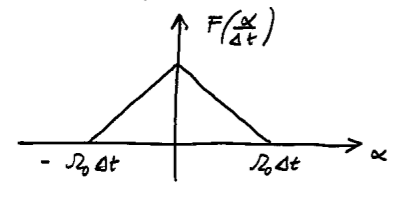
\includegraphics{figuras/12-0}
\end{figure}

Como $\Phi(\alpha)$ é uma combinação de $F(\alpha / \Delta t + k 2 \pi / \Delta
t)$ para diferentes valores de $k$ e o gráfico dessas funções são translações
por $k 2 \pi / \Delta t$ do gráfico de $F(\alpha / \Delta t)$, podemos ter uma
das situações abaixo:
\begin{figure}[htb]
  \centering
  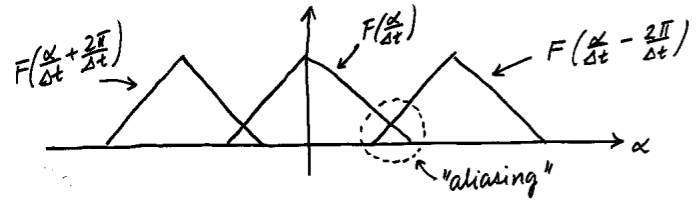
\includegraphics{figuras/12-1} \\
  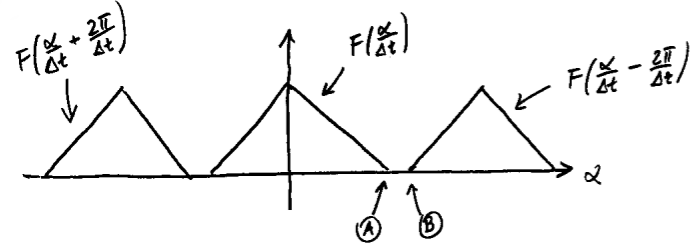
\includegraphics{figuras/12-2}
\end{figure}

É óbvio que apenas no segundo caso a soma dos perfis deslocados não altera o
perfil original. Note que nesse caso para os pontos $A$ e $B$ temos $x(B) - x(A)
\geq 0$. Se $F(x) = 0$ para $\lvert x \rvert \geq \Omega_0$, então $x(A) =
\Omega_o \Delta t$ e $x(B) = - \Omega_0 \Delta t + 2 \pi$, de modo que devemos
ter $-\Omega_0 \Delta t + 2 \pi - \Omega_0 \Delta t \geq 0$ e portanto
\begin{dmath*}
  \Omega_0 \Delta t \leq \pi.
\end{dmath*}
Além disso, camo $-\pi \leq \alpha \leq \pi$ e $x(\theta)$ nesse caso satisfaz
$x(\theta) \geq 2 \pi - \pi \geq \pi$, só temos a contribuição para
$\Phi(\alpha)$ da parte com $k = 0$, ou seja,
\begin{dmath*}
  \Phi(\alpha) = \frac{\sqrt{2 \pi}}{\Delta t} F\left( \frac{\alpha}{\Delta t} \right)
\end{dmath*}
se $F(x) = 0$, $\lvert x \rvert \geq \Omega_0$ e $\Omega_0 \Delta t \leq \pi$.
Nessas condições podemos reconstruir $f(t)$. De fato:
\begin{dmath*}
  f(t) = \frac{1}{\sqrt{2 \pi}} \int_{-\infty}^{+\infty} F(w) \exp(-i w t)
  \vi{w}
  = \frac{1}{\sqrt{2 \pi}} \int_{-\Omega_0}^{+\Omega_0} F(w) \exp(-i w t) \vi{w}
  = \frac{1}{\sqrt{2 \pi}} \int_{-\Omega_0 \Delta t}^{+\Omega \Delta t} F\left(
  \frac{\alpha}{\Delta t} \right) \exp(-i \alpha t / \Delta t)
  \frac{\vi{\alpha}}{\Delta t}
  = \frac{1}{2 \pi} \int_{-\Omega_0 \Delta t}^{+\Omega_0 \Delta t} \Phi(\alpha)
  \exp(-i \alpha t / \Delta t) \vi{\alpha}
  = \frac{1}{2 \pi} \int_{-\Omega_0 \Delta t}^{+\Omega_0 \Delta t} \left(
  \sum_{n = -\infty}^{+\infty} f_n \exp(i n \alpha) \right) \exp(-i \alpha t /
  \Delta t) \vi{\alpha}
  = \frac{1}{2 \pi} \sum_{n = -\infty}^{+\infty} f_n \left.
  \frac{\exp(i \alpha (n - t / \Delta t)}{i (n - t / \Delta t)}
  \right|_{-\Omega_0 \Delta t}^{+\Omega_0 \Delta t}
  = \frac{1}{\pi} \sum_{n = -\infty}^{+\infty} \frac{f_n}{(n - t / \Delta t)}
  \frac{\left[ \exp(i \Omega_0 \Delta t (n - t / \Delta t)) - \exp(-i \Omega_0
  \Delta t (n - t / \Delta t)) \right]}{2 i},
\end{dmath*}
ou seja,
\begin{dmath*}
  f(t) = \frac{\Delta t}{\pi} \sum_{n = -\infty}^{+\infty} f_n
  \frac{\sin(\Omega_0) (t - n \Delta t)}{t - n \Delta t}.
\end{dmath*}

Essa fórmula para reconstruir $f(t)$ á partir de $f_n$ é a essência do Teorema
da Amostragem de Shannon. Devemos lembrar as condições para que essa
reconstrução seja possível:
\begin{itemize}
  \item $F(w)$ deve ter suorte limitado ($F(w) = 0$ para $\lvert w \rvert \geq
    \Omega_0$), e
  \item o intervalo de amostragem deve satisfazer $\Delta t \leq \pi / \Omega_0$
    ou em termos da frequência de amostragem $\nu = 2 \pi / \Delta t$, $\nu \geq
    2 \Omega_0$.
\end{itemize}
A frequência $2 \Omega_0$ é chamada frequência de Nyquist. Podemos resumir nossa
situação através do diagrama:
\begin{figure}[htb]
  \centering
  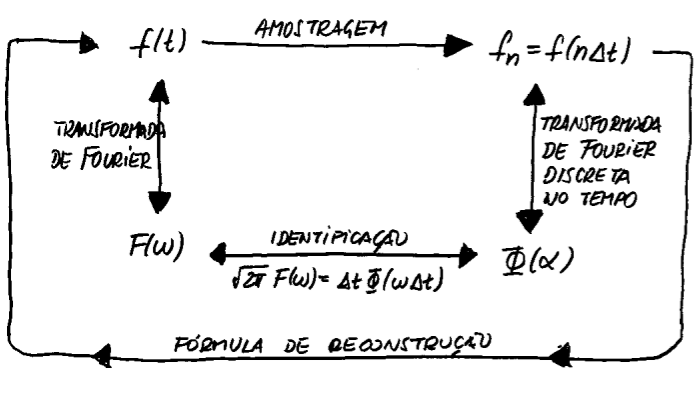
\includegraphics{figuras/12-3}
\end{figure}

\section{Transformada de Fourier Discreta}
Vamos agora estudar o caos em que temos apenas um número finito $f_0, f_1,
\ldots, f_{n - 1}$ de valores de $f(t)$ para o intervalo finito $[0, T]$, de
modo que dividindo o intervalo $[0, T]$ em $N$ pontos $t_k$,
\begin{dmath*}
  t_k = K T / N \condition{$k = 0, 1, \ldots, N - 1$,}
\end{dmath*}
temos $f_k = f(t_k)$.

Para isso vamos considerar a identidade
\begin{dmath*}
  q^N - 1 = (q - 1) (1 + q + q^2 + \ldots q^{N - 1}).
\end{dmath*}
Se $q^N = 1$ concluímos que $q^N - 1 = 0$ e portanto $q = 1$ ou $1 + q + \ldots
+ q^{N - 1} = 0$ se $q \neq 1$.

As raízes não triviais de $q^N = 1$ são da forma $\exp(n 2 \pi i / N)$, para $n
= 1, 2, \ldots, N - 1$, de modo que
\begin{dmath*}
  \sum_{k = 0}^{N - 1} q^k = \begin{cases}
    0, & \text{se } q = \exp(n 2 \pi i / N), n = 1, 2, 3, \ldots, N - 1, \\
    N, & \text{se } q = 1.
  \end{cases}
\end{dmath*}
Outra forma de escrevermos isso é fixando $q = \exp(2 \pi i / N)$ de modo que os
outros valores de $q$ são da forma $q^n$, $n = 0, 1, \ldots, N - 1$, e com isso
temos que
\begin{dmath*}
  \sum_{k = 0}^{N - 1} q^{n k} = N \delta_{n0},
\end{dmath*}
onde $\delta_{n0} = 0$ se $n \neq 0$ e $\delta_{n0} = 1$ se $n = 0$.

Definindo $w_n = n 2 \pi / T$ vemos que
\begin{dgroup*}
  \begin{dmath*}
    \exp(i w_n t_k) = \exp(i n (2 \pi / T) (k T / N))
    = \left( \exp(i 2 \pi / N) \right)^{n k}
    = q^{n k},
  \end{dmath*}
  \begin{dmath*}
    \left( \exp(i w_n t_k) \right)^k = \exp(-i w_n t_k)
    = q^{-n k}.
  \end{dmath*}
\end{dgroup*}
Com isso vemos que
\begin{dmath*}
  \sum_{k = 0}^{N - 1} \left( \exp(i w_n t_k) \right)^k \left( \exp(i w_m t_k)
  \right) = \sum_{k = 0}^{N - 1} q^{-n k} q^{m k}
  = \sum_{k = 0}^{N - 1} q^{(m - n) k},
  = N \delta_{mn}.
\end{dmath*}

Por outro lado,
\begin{dmath*}
  \sum_{n = 0}^{N - 1} \left( \exp(i w_n t_k \right)^k \exp(i w_n t_k) = \sum_{n
  = 0}^{N - 1} q^{-n k} q^{n l}
  = \sum_{n = 0}^{N - 1} q^{n (l - k)}
  = N \delta_{k l}.
\end{dmath*}

Isso nos sugere definir $F(w_n)$, $n = 0, 1, \ldots, N - 1$, como
\begin{dmath*}
  F(w_n) = \sum_{k = 0}^{N - 1} f(t_k) \exp(i w_n t_k).
\end{dmath*}
Com isso:
\begin{dmath*}
  \sum_{n = 0}^{N - 1} F(w_n) \left( \exp(i w_n t_l \right)^k = \sum_{n = 0}^{N
  - 1} \sum_{k = 0}^{N - 1} f(t_k) \exp(i w_n t_k) \exp(-i w_n t_l)
  = \sum_{k = 0}^{N - 1} f(t_k) \sum_{n = 0}^{N - 1} q^{n k} q^{-n l}
  = \sum_{k = 0}^{N - 1} f(t_k) N \delta_{kl}
  = N f(t_l),
\end{dmath*}
ou seja,
\begin{dmath*}
  f(t_k) = \frac{1}{N} \sum_{n = 0}^{N - 1} F(w_n) \exp(-i w_n t_k).
\end{dmath*}

Portanto $F(w_n)$ é a transformada de Fourier discreta e $f(t_k)$ a sua
transformada inversa.

Podemos notar que
\begin{dmath*}
  F(w_n) = \sum_{k = 0}^{N - 1} f(t_k) g^{n k}
\end{dmath*}
pode ser escrita numa forma matricial, ou seja,
\begin{dmath*}
  F = Q_N f,
\end{dmath*}
onde $Q_N$ é chamada matriz de Fourier,
\begin{dmath*}
  \begin{bmatrix}
    F(w_0) \\
    F(w_1) \\
    \vdots \\
    F(w_{N - 1})
    \end{bmatrix} = \begin{bmatrix}
    q^{00} & q^{01} & \ldots & q^{0(N - 1)} \\
    q^{10} & q^{11} & \ldots & q^{1(N - 1)} \\
    \vdots & \vdots & \ddots & \vdots \\
    q^{(N - 1)0} & q^{(N - 1)1} & \ldots & q^{(N - 1)(N - 1)}
  \end{bmatrix} \begin{bmatrix}
    f(t_0) \\
    f(t_1) \\
    \vdots \\
    f(t_{N - 1})
  \end{bmatrix}
\end{dmath*}

Como podemos ver, a matriz $Q_N$ apresenta uma grande redundância. De fato:
\begin{dmath*}
  Q_N =  \begin{bmatrix}
    1 & 1 & 1 & \ldots & 1 \\
    1 & q^{1} & q^{2} & \ldots & q^{(N - 1)} \\
    1 & q^{2} & q^{4} & \ldots & q^{2(N - 1)} \\
    \vdots & \vdots & \vdots & \ddots & \vdots \\
    1 & q^{(N - 1)} & q^{2 (N - 1)} & \ldots & q^{(N - 1)(N - 1)}
  \end{bmatrix}
\end{dmath*}

Podemos eliminar um pouco dessa redundância através de um algoritmo chamado
``transformada de Fourier rápida''\footnote{Em inglês, Fast Fourier Transform ou
FFT.}. Para isso é essencial que o número de pontos seja $2^n$, ou seja, $N =
2^n$. Vamos ainda denotar $N_k = 2^{n - k}$ de modo que $N = 2^K N_k$, $k = 0,
1, \ldots, n$.

Considerando $F(w_n)$, podemos escrever ($N = 2 N_1$)
\begin{dmath*}
  F(w_n) = \sum_{k = 0}^{N - 1} f(t_k) g^{n k}
  = \sum_{k = 0}^{N_1 - 1} f(t_k) g^{n k} + \sum_{k = N_1}^{2 N_1 - 1} f(t_k)
  q^{n k}
  = \sum_{k = 0}^{N_1 - 1} f(t_k) g^{n k} + \sum_{k = 0}^{N_1 - 1} f(t_{(k +
  N_1)}) q^{n (k + N_1)}.
\end{dmath*}
Mas
\begin{dmath*}
  q = \exp(2 \pi i / N)
  = \exp(2 \pi i / (2 N_1))
  = \exp(\pi i / N_1),
\end{dmath*}
ou seja, $q^{N_1} = \exp(\pi i) = -1$ e $q^{n N_1} = (-1)^n$. Logo:
\begin{dmath*}
  F(w_n) = \sum_{k = 0}^{N_1 - 1} f(t_k) q^{n k} + \sum_{k = 0}^{N_1 - 1} f(t_{k
  + N_1}) g^{n k} (-1)^n
  = \sum_{k = 0}^{N_1 - 1} \left[ f(t_k) + (-1)^n f(t_{k + N_1}) \right] g^{n
  k}.
\end{dmath*}
De modo que
\begin{dgroup*}
  \begin{dmath*}
    F(w_{2 n_1}) = \sum_{k = 0}^{N_1 - 1} \left[ f(t_k) + f(t_{k + N_1}) \right]
    \left( q^2 \right)^{k n_1},
  \end{dmath*}
  \begin{dmath*}
    F(w_{2 n_1 + 1}) = \sum_{k = 0}^{N_1 - 1} \left[ f(t_k) - f(t_{k + N_1})
    \right] \left( q^2 \right)^{K n_1} q^k,
  \end{dmath*}
\end{dgroup*}
para $n_1 = 0, 1, \ldots, N_1 - 1$.

Como a matriz $Q_N$ é $N \times N = 2^n 2^n = 2^{2n}$, agora temos $2 N_1 N_1 =
2 2^{n - 1} 2^{n - 1} = 2^{2 n - 1}$, ou seja, o número de operações
(multiplicações) é reduzido pela metade.

Uma forma de olhar para o procedimento acima é notando que
\begin{dmath*}
  q^2 = \left( \exp(2 \pi i / N) \right)^2
  = \exp(2 \pi i / (N / 2))
  = \exp(2 \pi i / N_1)
  = q_1,
\end{dmath*}
ou seja, $(q^2)^{k n_1}$, $k_1 n_1 = 0, 1, \ldots, N_1 - 1$, são entradas da
matriz de Fourier para $N_1$, ou seja,
\begin{dmath*}
  \begin{bmatrix}
    F(w_0) \\
    F(w_1) \\
    \vdots \\
    F(w_{2 N_1 - 1})
  \end{bmatrix} =  \begin{bmatrix}
    1 & 1 & \ldots & 1 \\
    1 & q^{2} & \ldots & q^{(N - 1)} \\
    1 & q^{4} & \ldots & q^{2(N - 1)} \\
    \vdots & \vdots & \ddots & \vdots \\
    1 & q^{2 (N - 1)} & \ldots & q^{(N - 1)(N - 1)}
  \end{bmatrix} \begin{bmatrix}
    f(t_0) + f(t_{N_1}) \\
    f(t_1) + f(t_{N_1 + 1})\\
    \vdots \\
    f(t_{N - 1}) + f(t_{2 N_1})
  \end{bmatrix}
\end{dmath*}

% TODO Terminar M2S12-12.pdf. Interrompido na página 15.
